\documentclass{beamer}
 
\usepackage[utf8]{inputenc}
\usepackage{animate}
 
\title{Propagation of Voltage in a Neuron}
\subtitle{The Cable Equation}
\author{Darice Guittet, Elise Niedringhaus, Sarah Liddle}
\date{Fall 2017}
 
 
 
\begin{document}
 
\frame{\titlepage}
 
\begin{frame}
\frametitle{Overview}
1. Motivation \newline \newline
2. Neuronal Cable Equation \newline \newline
3. Passive Membrane \newline \newline
4. Bi-stable Ion Channels
\end{frame}

\begin{frame}
\frametitle{How Do Neurons Communicate?}
\begin{columns}
    \begin{column}{.5\textwidth}
    Within one cell
    \begin{itemize}
	\item Electrochemical signals
	\item Membrane Potential: $\Delta V_m = V_i - V_e$
	\item Ions: charge-carriers
	\item Ion Channels in Membrane \newline
	\end{itemize}
	Between cells
	\begin{itemize}
	\item Neurotransmitters
\end{itemize}
    \end{column}
    
    \begin{column}{.5\textwidth}
    \begin{figure}[H]\label{neuron}
    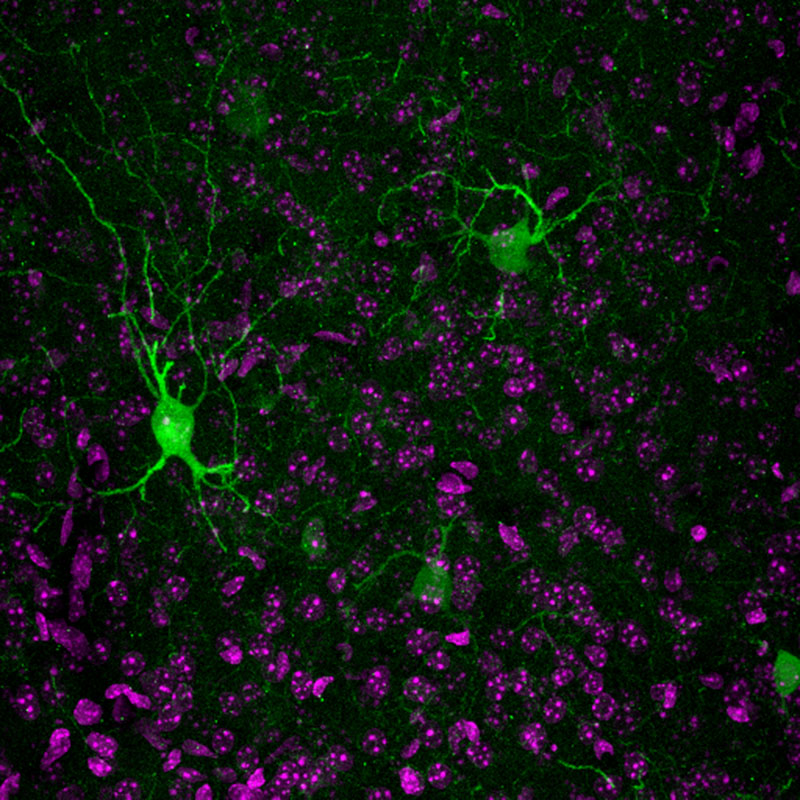
\includegraphics[width=\textwidth]{OConnor-InhibitoryInterneurons1}
	\caption{Mouse neurons, 40X. Bosch Institute Advanced Microscopy Facility, The University of Sydney}
    \end{figure}
    
    \end{column}
  \end{columns}
\end{frame}

\begin{frame}
\frametitle{Action Potentials}
\begin{figure}
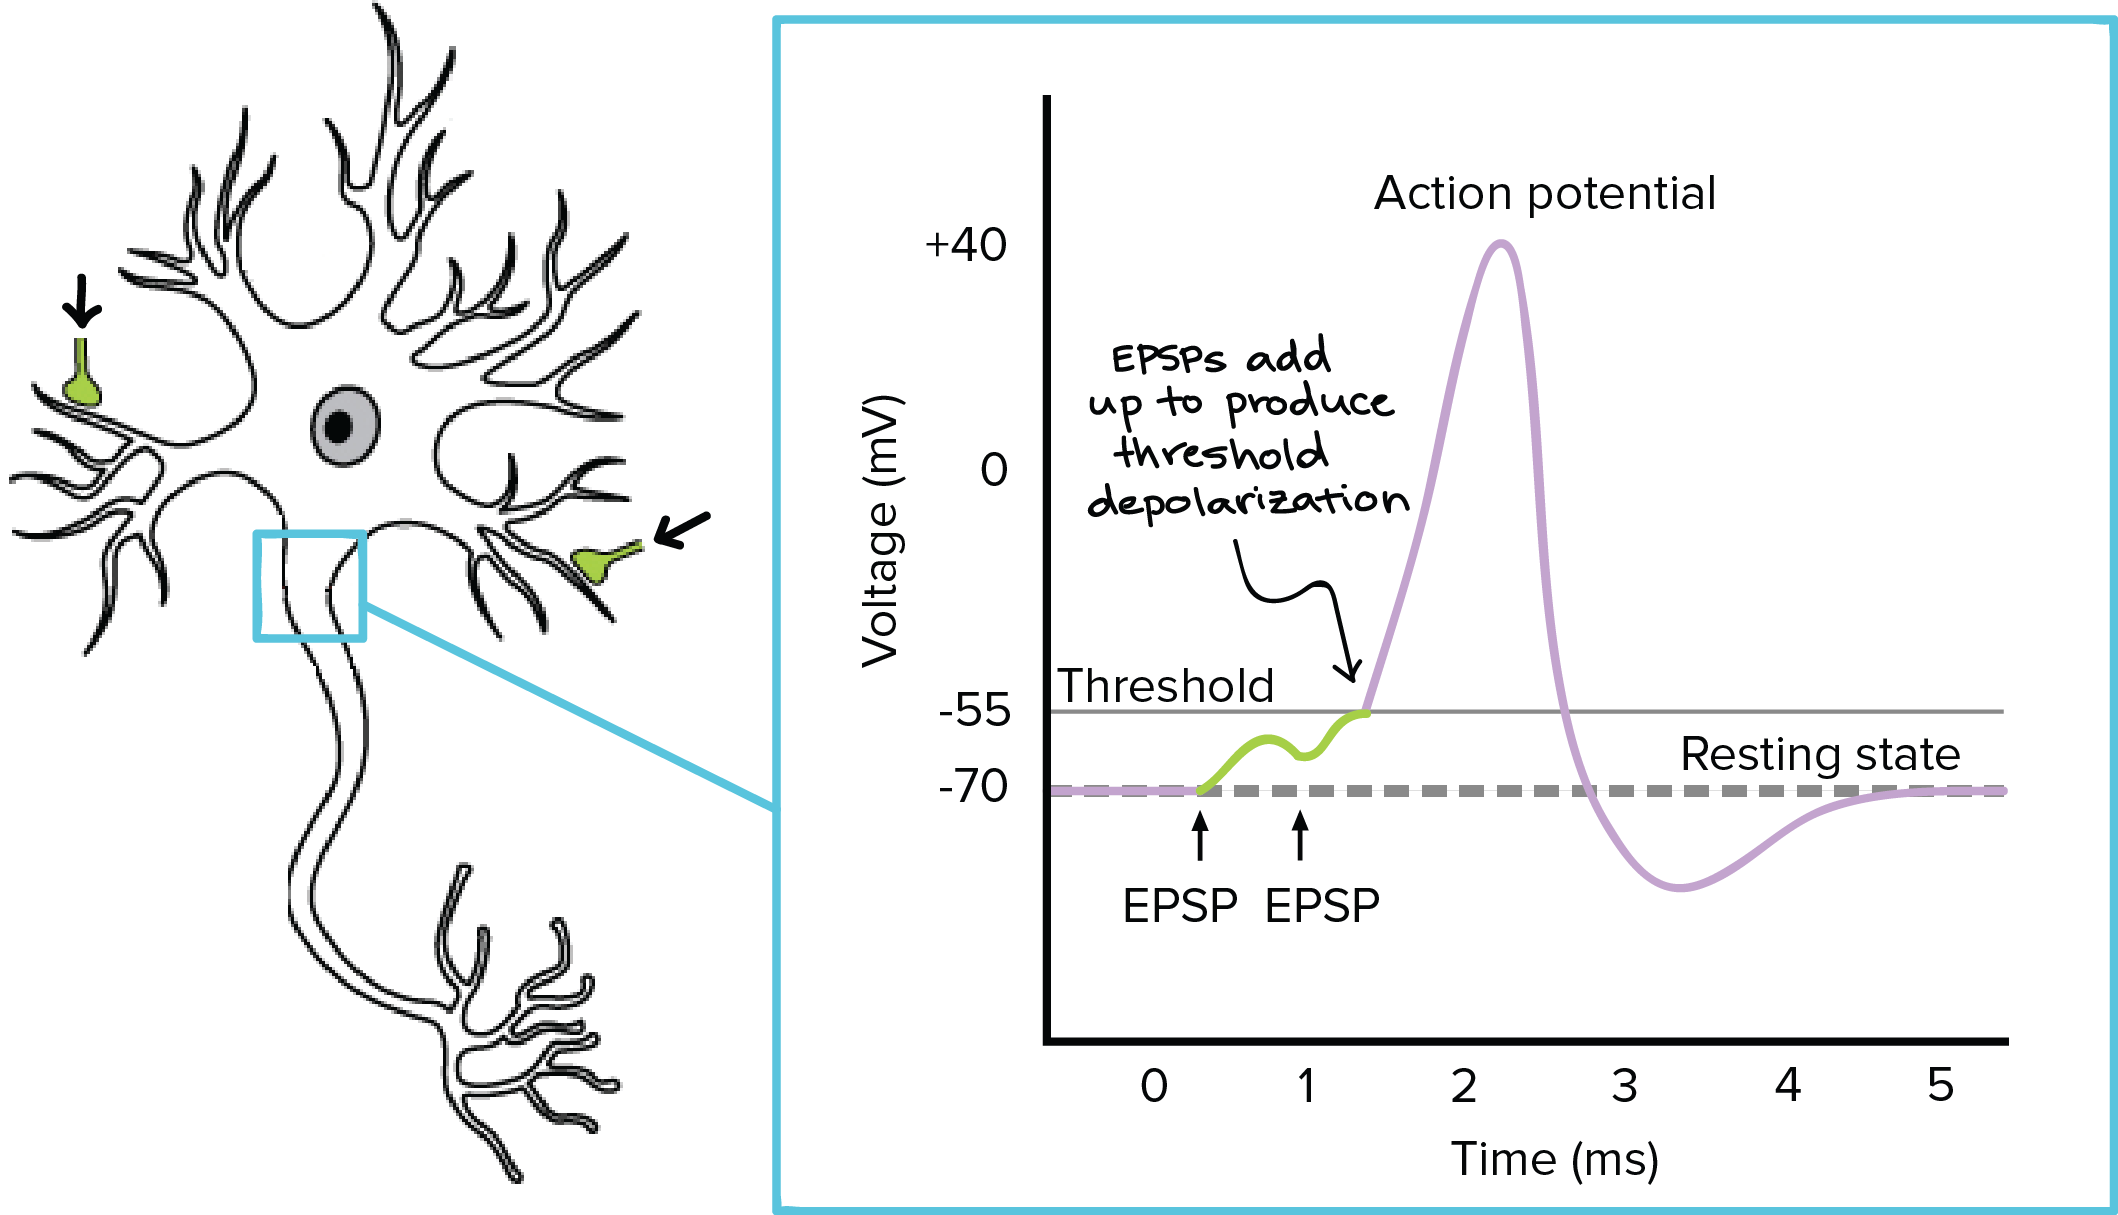
\includegraphics[width=\textwidth]{actionpotential}
\caption{Changes in axonal membrane voltage due to an action potential. Image from Khan Academy}
\end{figure}
\end{frame}

\begin{frame}
\frametitle{Hodgkin-Huxley's Neuronal Cable Model}
\begin{columns}
\begin{column}{.65\textwidth}
\begin{figure}
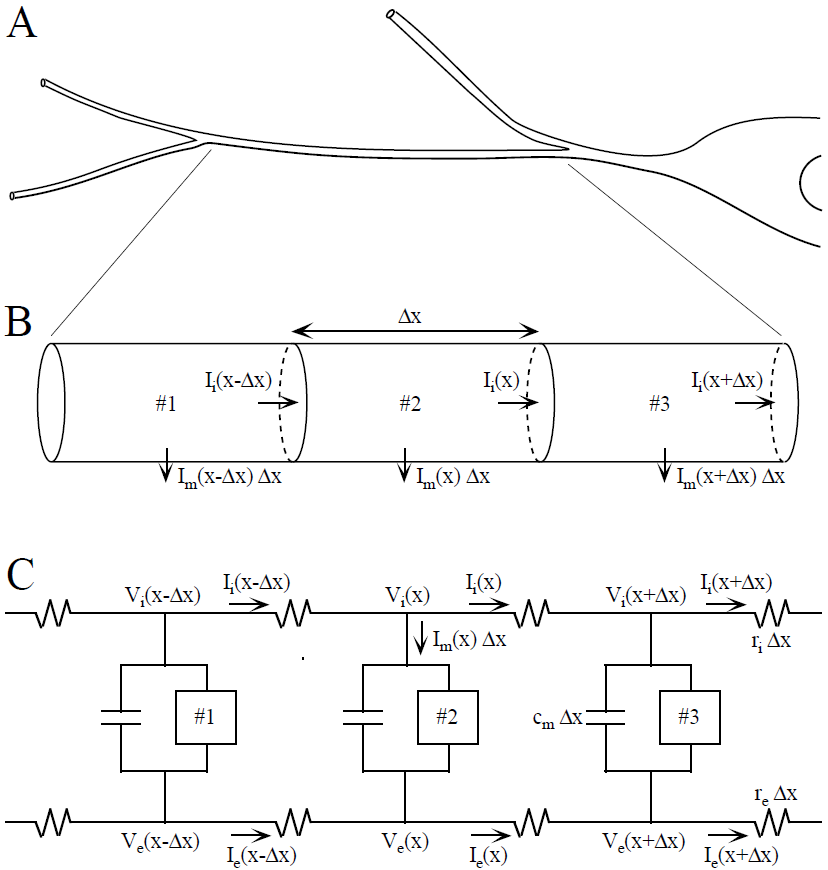
\includegraphics[scale=0.35]{NeuronalCableModel}
\caption{Differential membrane patches as circuit. Image from jh.edu/motn}
\end{figure}
\end{column}

\begin{column}{.45\textwidth}
\begin{itemize}
	\item{1-D \& Ohmic assumption}
	\item{Intracellular current}
	\item{Extracellular current}
	\item{Membrane current}
	\item{Membrane as capacitor}
	\item{Ion channels as conductances}
	\item{Length Constant: $\lambda = \sqrt{\frac{r_m}{r_i+r_e}}$}
	\item{Time Constant: $r_mC_m$ }
\end{itemize}
\end{column}
\end{columns}
\end{frame}




\begin{frame}
\frametitle{Passive Membrane}
Linear Cable Equation with Impulse Current Injection:

$$\frac{\partial{v(x,t)}}{\partial{t}} - \frac{\partial^2{v(x,t)}}{\partial{x}^2} + v(x,t)=\delta(t-t_0)\delta(x-x_0)$$ 

$$x \in (-\infty, \infty),\ t \in (0,\infty),\ x_0 = 0,\ t_0 = 0$$ \newline

Boundary Conditions:
$$\lim_{x\to \pm \infty} v(x,t) = 0$$
\end{frame}

\begin{frame}
\frametitle{Green's Function for Linear Infinite Cable Equation}
Fourier transform $\rightarrow$ 2 ODE's $\rightarrow$ Inverse Fourier transform
$$ v(x,t) = \frac{\mathcal{H}(x,t)}{\sqrt{4\pi t}}e^{-t-\frac{x^2}{4t}} $$ 

$$  G_{\infty}(x-x_0,t-t_0) = \frac{\mathcal{H}(x-x_0,t-t_0)}{\sqrt{4\pi (t-t_0)}}e^{-(t-t_0)-\frac{(x-x_0)^2}{4(t-t_0)}}$$\newline

Fundamental Solution for Arbitrary Forcing Term, $J_{ext}(x,t)$:
$$ \hat{v}(x,t) = \int_{-\infty}^{\infty}\int_{-\infty}^{\infty}G_{\infty}(x-x_0,t-t_0)J_{ext}(x_0,t_0)dx_0dt_0 $$
\end{frame}

\begin{frame}
\frametitle{Multiple Current Injections: $(x^*,t^*,A^*) = (1, 0.3, 0.3), (10,1.1,1), (30,0,0.5)$}
	\animategraphics[controls,autoplay,loop, width=1\linewidth]{5}{pm/pm-}{0}{49}
	
\end{frame}

\begin{frame}
\frametitle{animation of traveling wave solution}
	\animategraphics[controls,autoplay,loop, width=1\linewidth]{10}{tw/tw-}{0}{100}
\end{frame}

\begin{frame}
\frametitle{animation of perturbed wave solution}
	\animategraphics[controls,autoplay,loop, width=1\linewidth]{10}{pt/pt-}{0}{99}
\end{frame}

\begin{frame}
\frametitle{Numerical Solutions}
\begin{itemize}
	\item{Finite Difference Method}
	\item{Plugging approximations for the partial derivatives into the original PDE gives:}
\[\frac{v^{j+1}_i-v^j_i}{\Delta{t}}=\frac{v^{j}_{i+1}-2v^j_i+v^j_{i-1}}{(\Delta{x})^2}-v^j_i+J_{ext}(x,t)\]
	\item{Solving for the unknown term:}
\[v^{j+1}_i=\frac{\Delta{t}}{(\Delta{x})^2}(v^{j}_{i+1}+v^{j}_{i-1})+(1-\frac{\Delta{t}(2+(\Delta{x})^2)}{(\Delta{x})^2})v^{j}_{i}+\Delta{t}*J_{ext}(x,t)\]
	\item{Stability}
\end{itemize}

\end{frame}

\begin{frame}
\frametitle{Numerical Solutions Results}
\begin{figure}[H]
  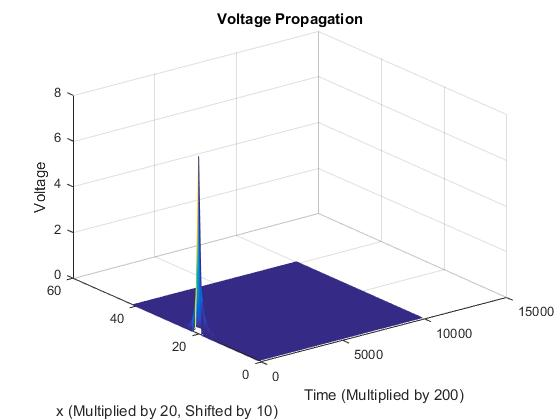
\includegraphics[width=\linewidth]{Plot2.jpg}
  \caption{Numerical Approximation of Passive Membrane Solution}
  \label{fig:sketch2}
\end{figure}
\end{frame}

\begin{frame}
\frametitle{Traveling Wave Solutions}
lalalala
\end{frame}

\begin{frame}
\frametitle{Speed of Traveling Wave}
lalalala
\end{frame}

\begin{frame}
\frametitle{Stability of Traveling Wave}
lalalala
\end{frame}

\begin{frame}
\frametitle{Numerical Solutions for Traveling Wave}
\begin{itemize}
	\item{Finite Difference Method--Similar to Previous Numerical Solution}
	\item{Resultant Equation (solved for the unknown term):}
\end{itemize}
\[v^{j+1}_i=\frac{\Delta{t}}{(\Delta{x})^2}(v^{j}_{i+1}+v^{j}_{i-1})+(1-\frac{\Delta{t}(2+(\Delta{x})^2)}{(\Delta{x})^2})v^{j}_{i}+\Delta{t}*H(v^j_i-\theta)\]


\end{frame}

\begin{frame}
\frametitle{Results}

\begin{columns}


\begin{column}{.5\textwidth}
\begin{figure}[H]
  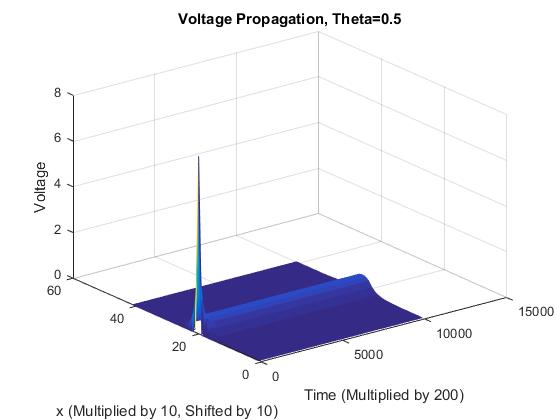
\includegraphics[width=\linewidth]{thetatwo.jpg}
  \caption{$\theta=0.5$}
  \label{fig:sketch5}
\end{figure}
\end{column}

\begin{column}{.5\textwidth}
\begin{figure}[H]
  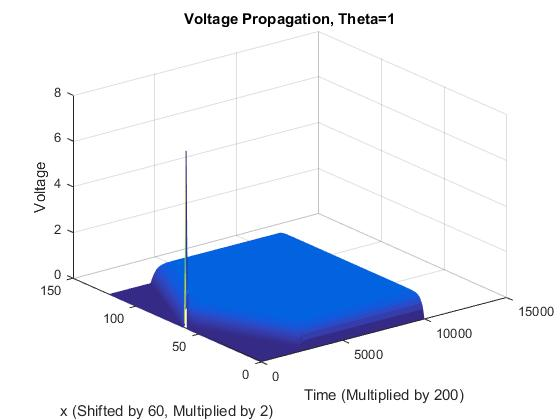
\includegraphics[width=\linewidth]{thetathree.jpg}
  \caption{$\theta=0.1$}
  \label{fig:sketch6}
\end{figure}
\end{column}

\end{columns}
\begin{itemize}
	\item{Numerically Solving for Speeds of the Waves}
	\item{Comparison with Analytic Results}
\end{itemize}
\end{frame}



%%%I might take this out, I'm not sure if we need it since it's not a solution we actually found analytically, it might be least important
\begin{frame}
\frametitle{Periodically Varying Threshold, Numerical Methods}
\begin{itemize}
	\item{What is a periodically varying threshold?}
	\item{Governing Equation:}
\[\frac{\partial{v(x,t)}}{\partial{t}}=\frac{\partial^2{v(x,t)}}{\partial{x}^2}-v+H(v-\theta(1+0.5\cos(x)))+J_{ext}(x,t)\]
	\item{Numerical Solution:}
\[v^{j+1}_i=\frac{\Delta{t}}{(\Delta{x})^2}(v^{j}_{i+1}+v^{j}_{i-1})+(1-\frac{\Delta{t}(2+(\Delta{x})^2)}{(\Delta{x})^2})v^{j}_{i}\]
\[+\Delta{t}*H(v^j_i-\theta(1+C\cos(x)))\]
\end{itemize}
\end{frame}


\begin{frame}
\frametitle{Results}
\begin{figure}[H]
  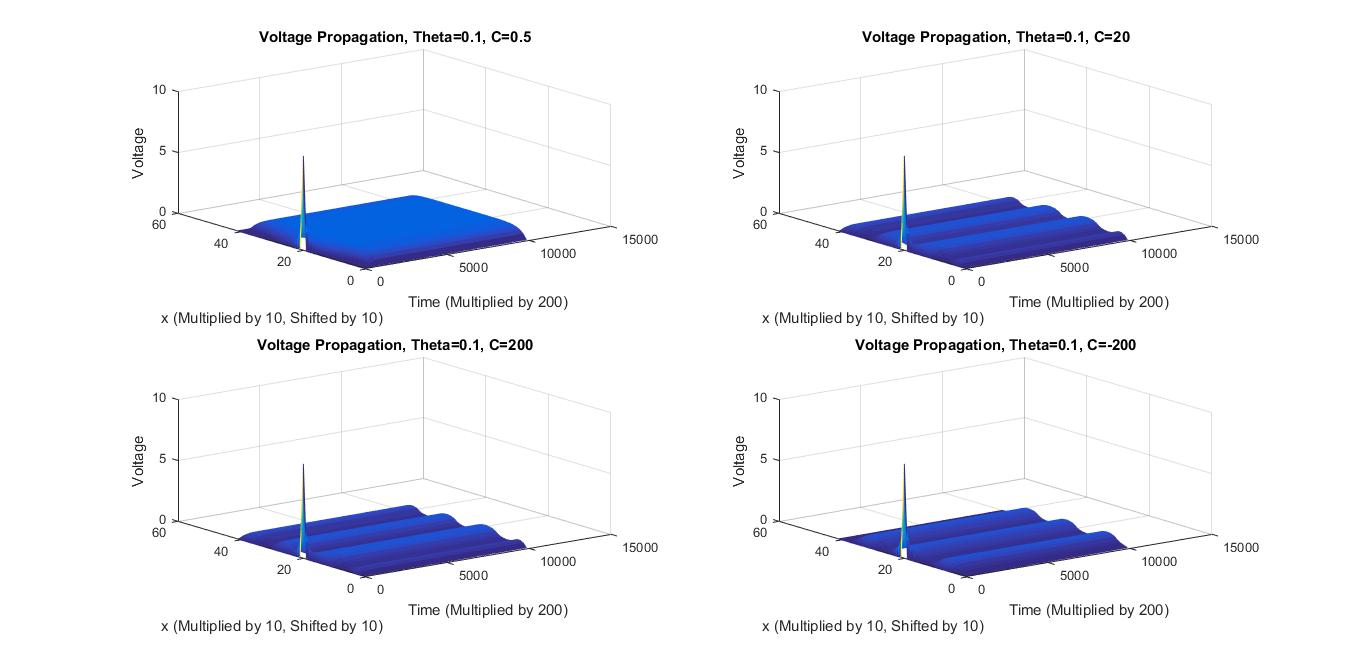
\includegraphics[width=\linewidth]{plotsomething.jpg}
  \caption{Varying $C$, $\theta=0.1$}
  \label{fig:sketch10}
\end{figure}
\end{frame}
%%%%%



\begin{frame}
\frametitle{Conclusion: Comparison to full Hodgkin-Huxley Model} 
\hfill \break
Three gating variables $x = m,n,h$, each satisfying ODE's:
$$ C\frac{\partial{v}}{\partial{t}} = g_{\text{Na}}m^3h(v-E_{\text{Na}})+g_{\text{K}}n^4(v-E_{\text{K}})+g_{\text{L}}(v-E_\text{L}) + J_{ext}$$
$$ \frac{dx}{dt} = -\frac{1}{\tau_x(v)}\big[x-x_0(v)\big] $$
\begin{figure}
	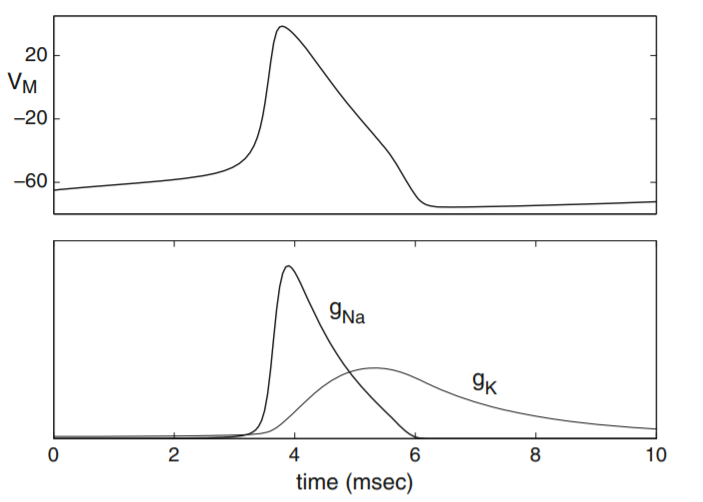
\includegraphics[scale=0.4]{conc/sol}
\end{figure}
\end{frame}
\end{document}